\mojesekce{Results}

\subsection{Sensitivity analyses}
\begin{block}{Sensitivity analyses}
\justifying
Each optimized parameter were increased and decreased with specific factor unit sum of squares increased with order of magnitude.  Functionalities of python package Scipy were used to perform optimization \citep{scipy}.
\begin{columns}
        \begin{column}{0.25\textwidth}
            \begin{itemize}
                \item screening: each parameter changed with factor and compared to optimized set of parameters 
                \item sum of squares for comparison
                \item sensitivity of eq. \ref{eq:manning} and infiltration parameters were tested
            \end{itemize}
        \end{column}
    \begin{column}{0.25\textwidth}
        \begin{table}[]
            \small
            \begin{tabular}{lll}
                \hline
                \hline
                Paraneter & increase   & decrease \\
                          & factor (+) & factor (-) \\
                \hline
                X         & 80                  & 1/3.5               \\
                Y         & 1.3                 & 1/1.6               \\
                b         & 1.125               & 1/1.5               \\
                Ks        & 2.0                 & 1/5.0               \\
                S         & 2.0                 & 1/5.0               \\
                ret       & 1.5                 & 1/5.0              \\
                \hline
                \hline
            \end{tabular}
        \end{table}
    \end{column}
    \begin{column}{0.5\textwidth}
        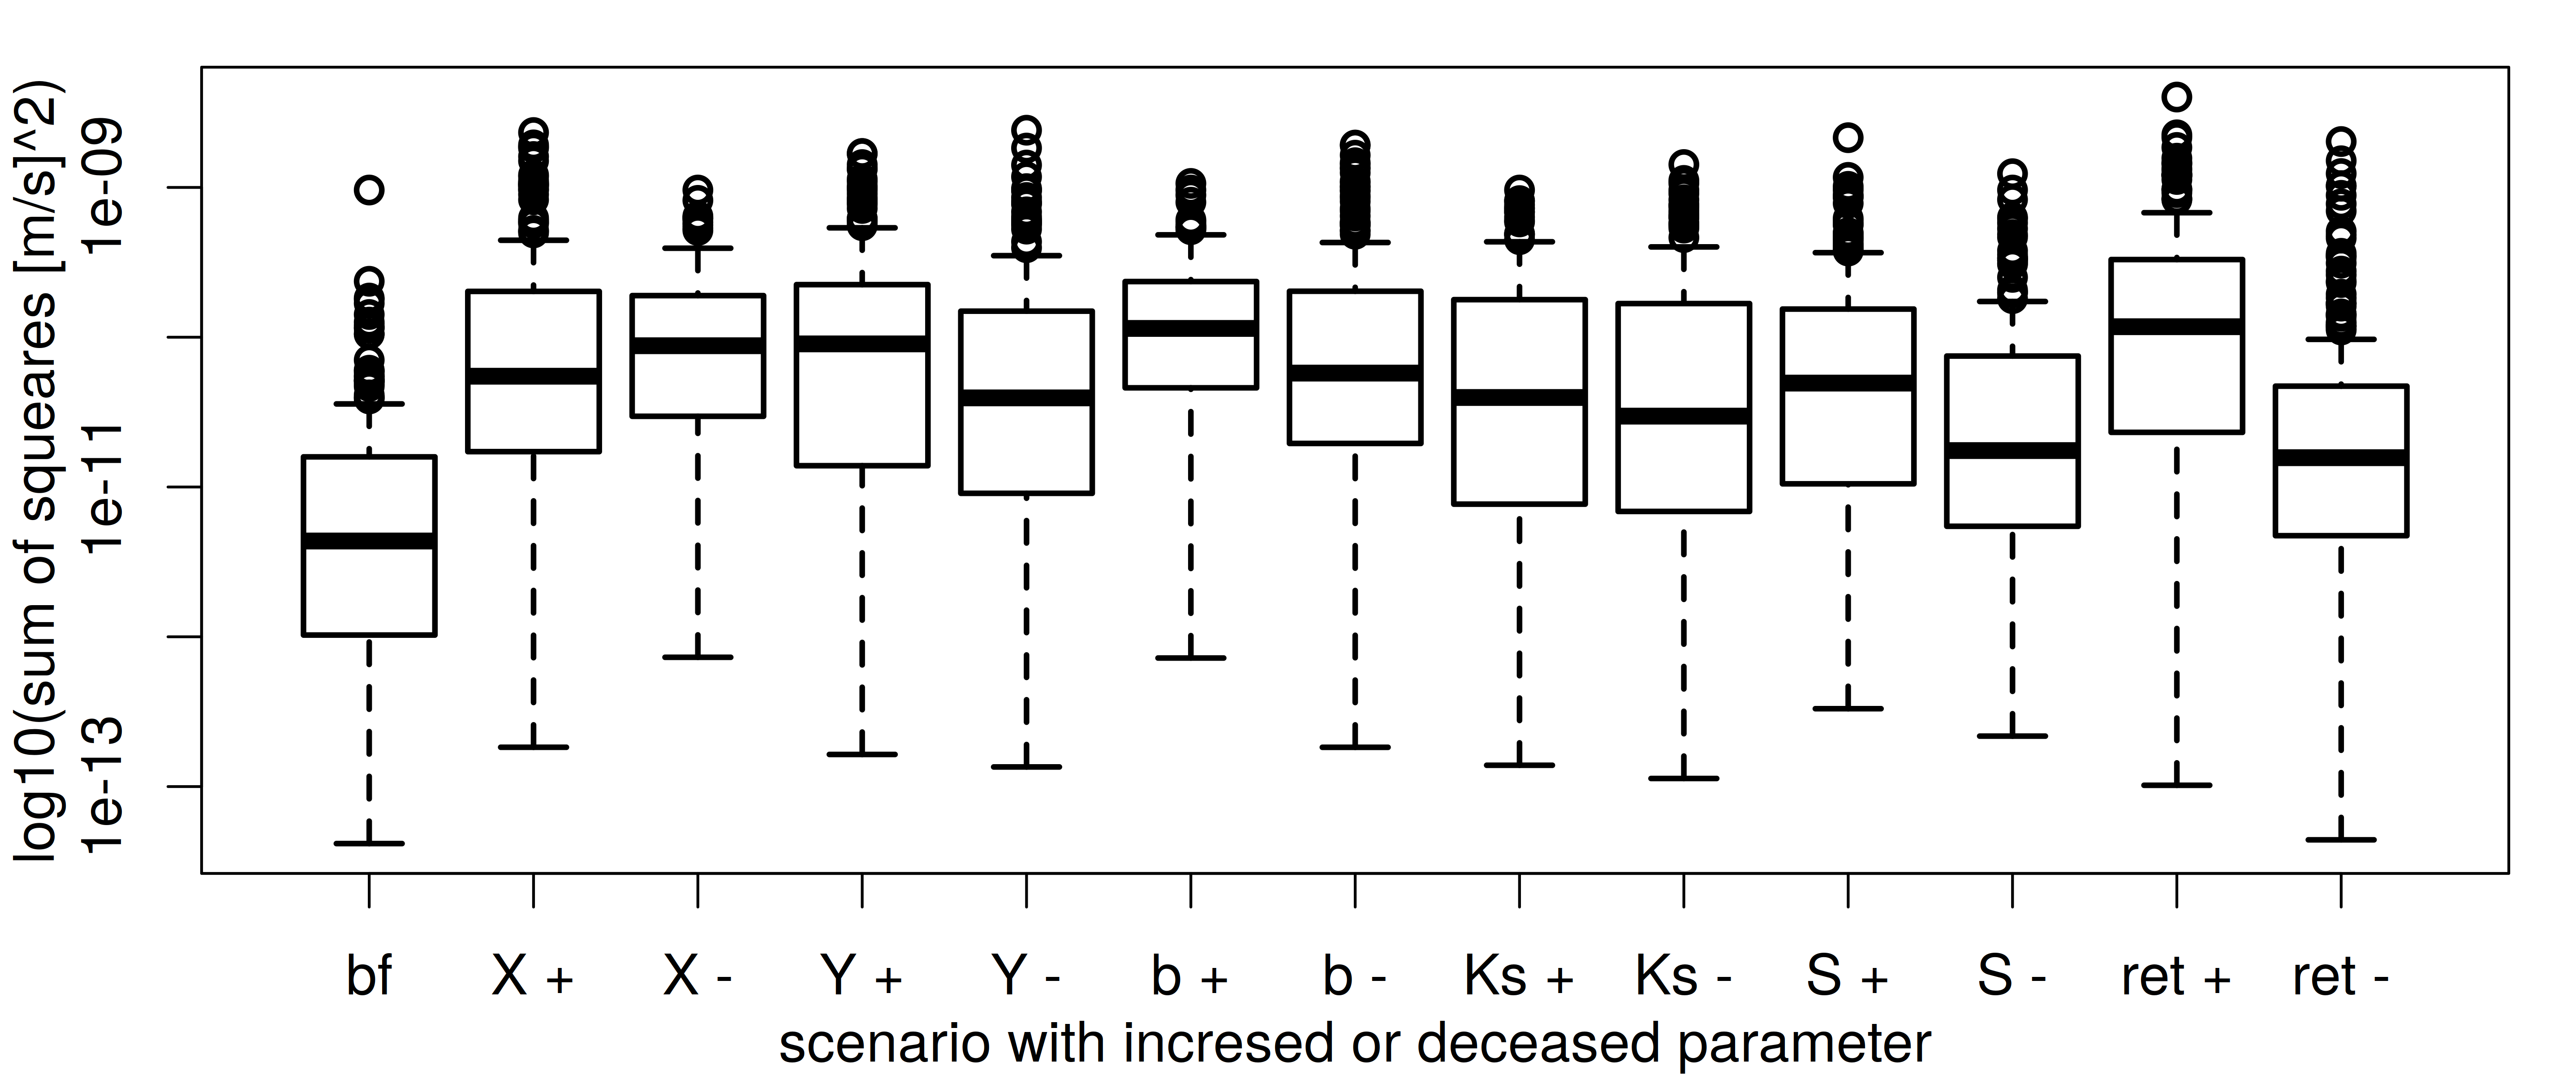
\includegraphics[width = \textwidth]{obr/sens.png}
    \end{column}
\end{columns}
\end{block}

% 
\subsection{Model parameters and textural classes}
\begin{block}{Model parameters and textural classes}
\begin{columns}
    \begin{column}{0.2\textwidth}
            \begin{itemize}
                \item infiltration parameters fitted with data
                \item differential evolution were used
                \item eq. \ref{eq:manning} parameters were optimized
                \item each experiment was optimized separately
            \end{itemize}
        \begin{table}[]
            \small
            \begin{tabular}{lllll}
            parameter: & X & Z & b & ret \\
            max & 30 & 5 & 4 & 0 \\
            min & 1 & 0.01 & 1 & -0.5 \\
            \end{tabular}
        \end{table}
    \end{column}
    \begin{column}{0.8\textwidth}
        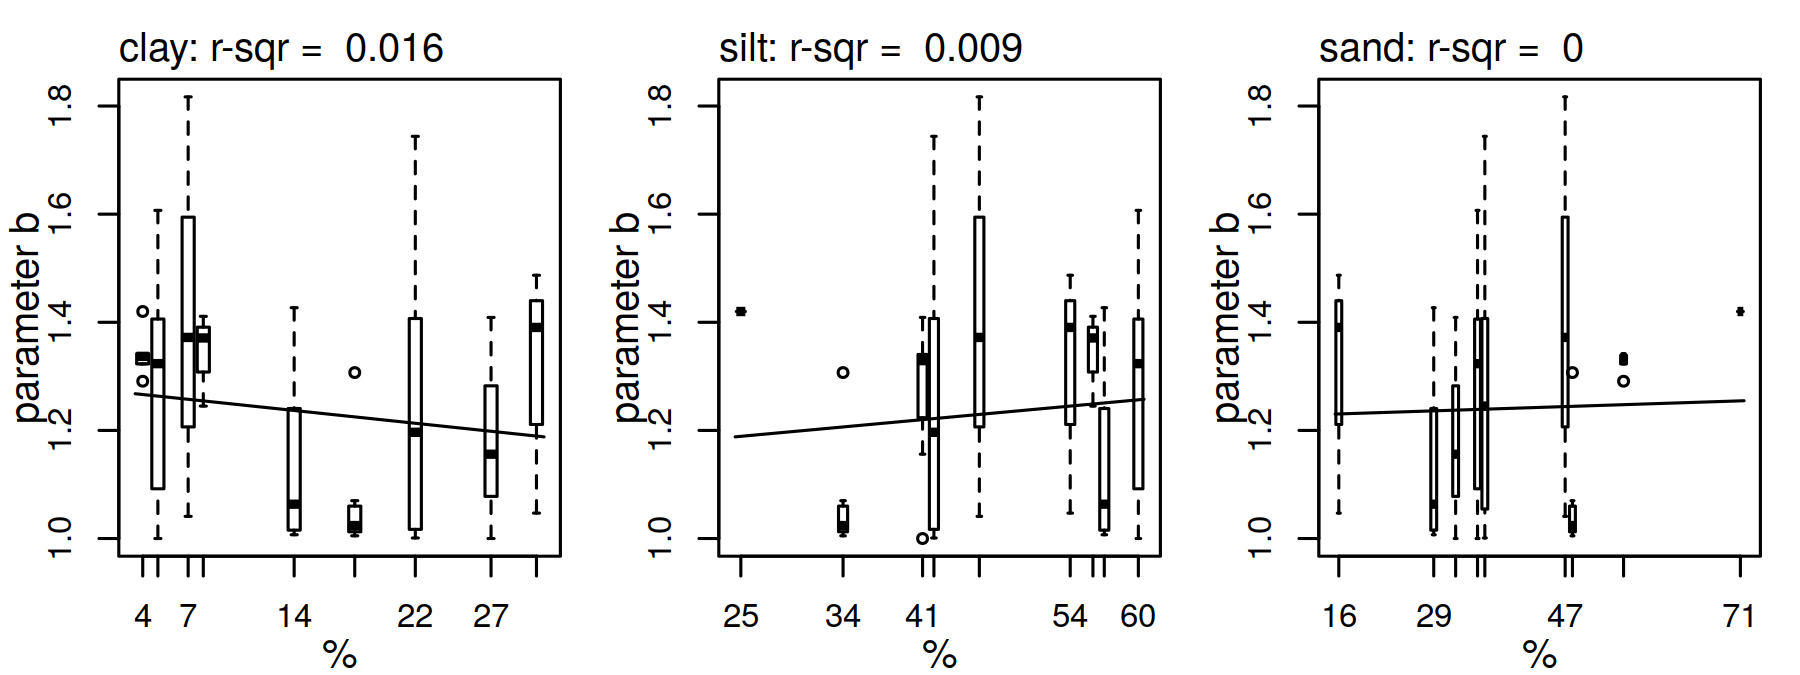
\includegraphics[width = \textwidth]{obr/bfittex.png}\\
        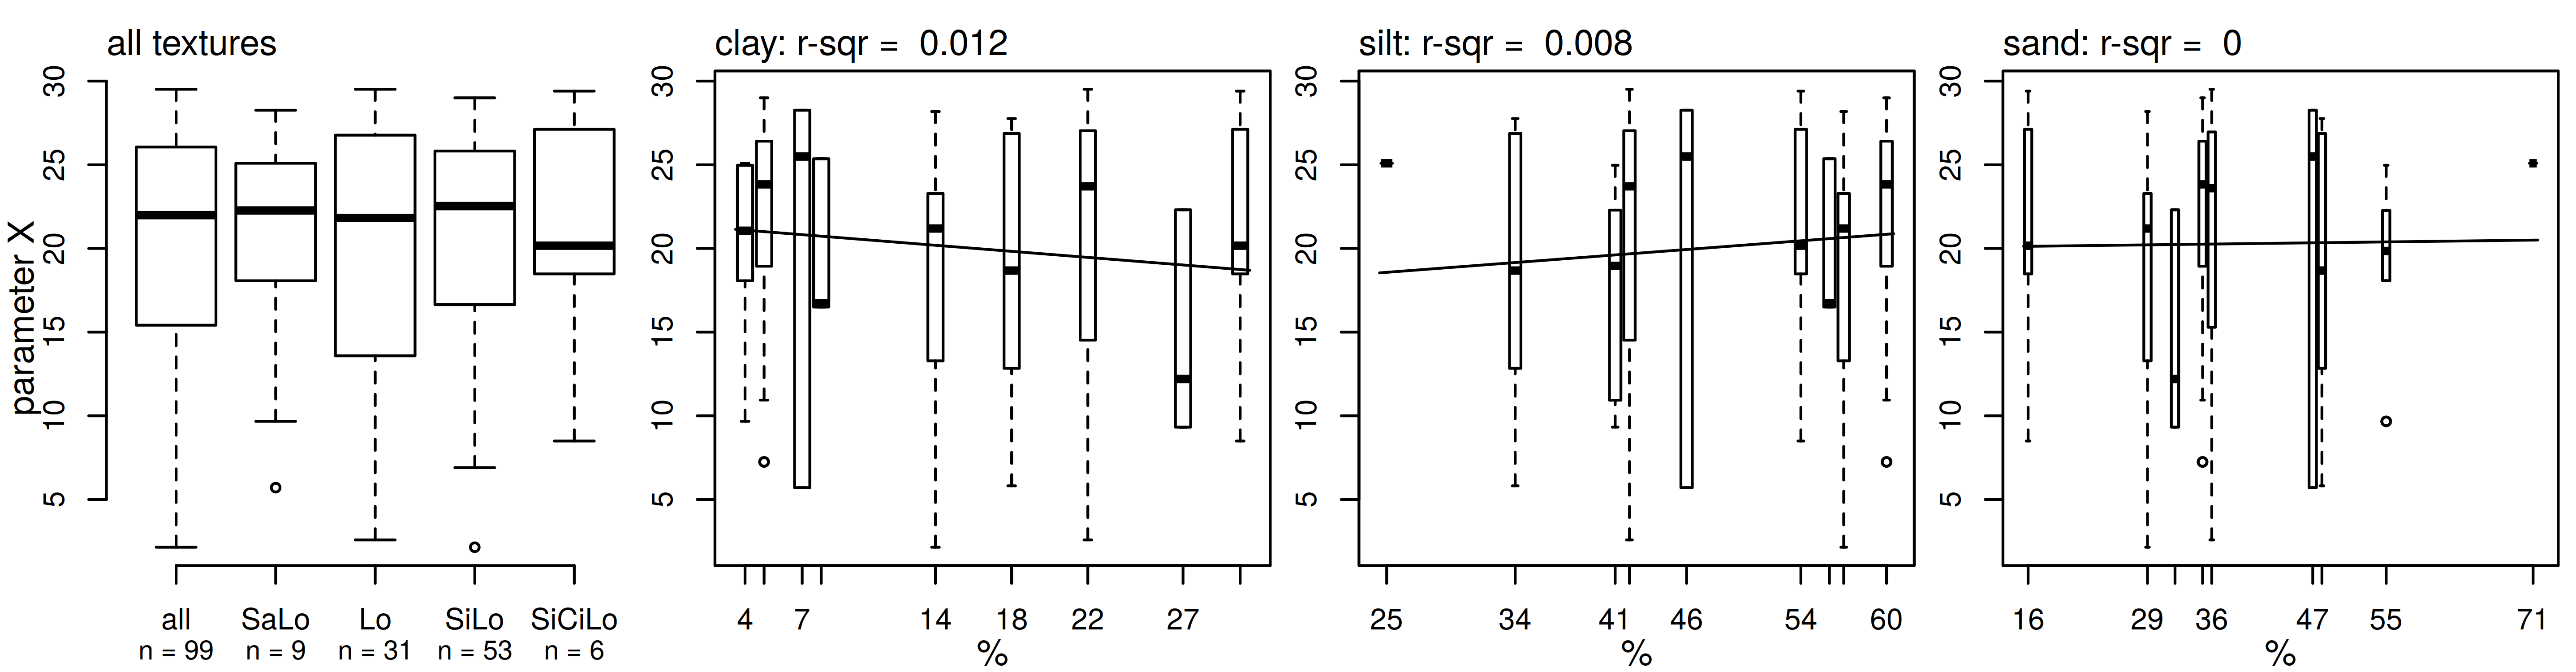
\includegraphics[width = \textwidth]{obr/Xfittex.png}\\
        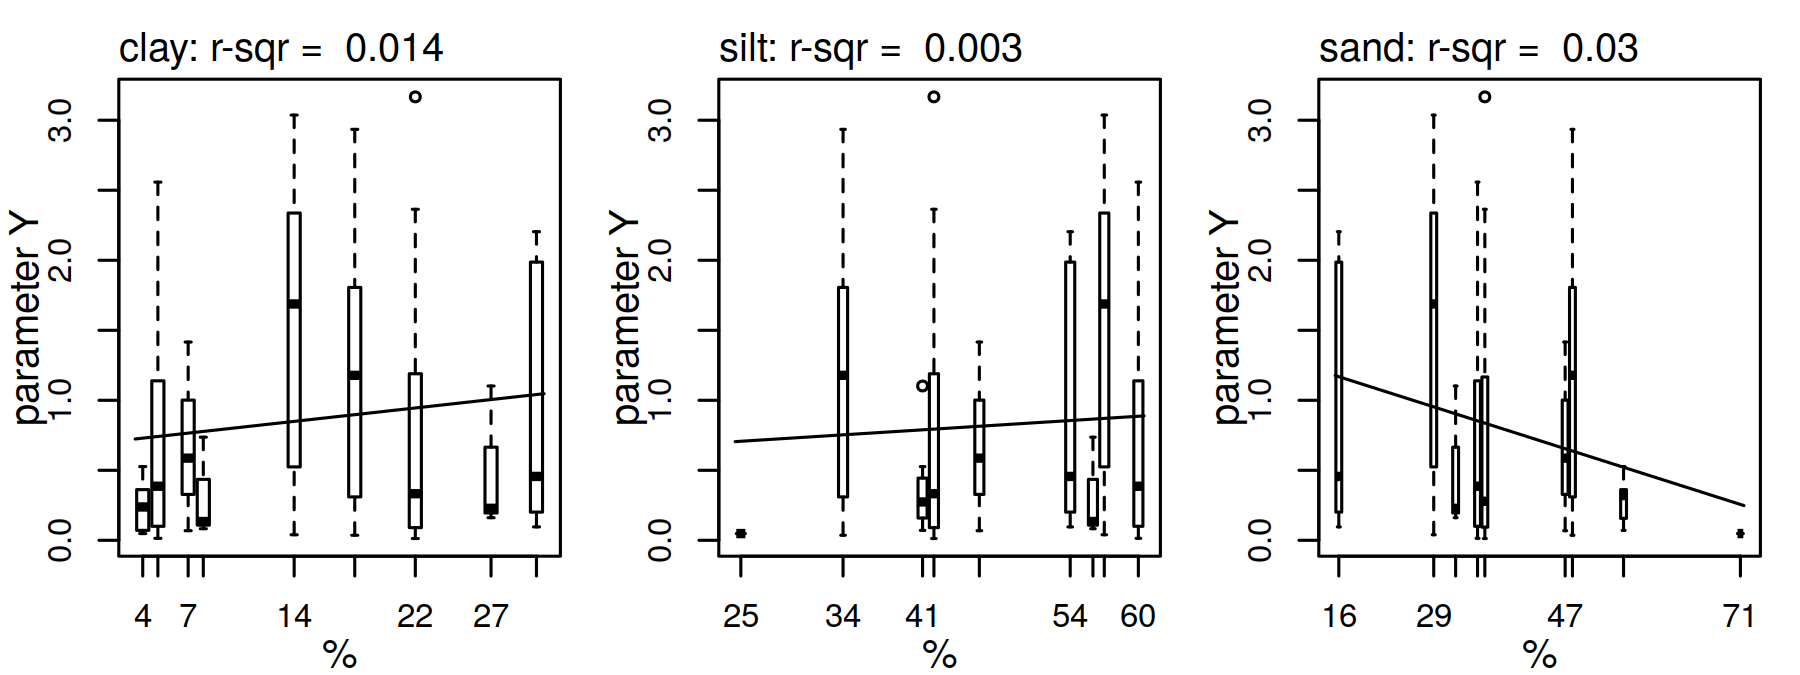
\includegraphics[width = \textwidth]{obr/Yfittex.png}
        {\it Figures shown optimized parameters. Top bar shown retults of parameter b, middle bar shown retults of parameter Y, and bottom bar shown retults of parameter Y. Left graph shows values for textural calss. Second to fourth graph shows parameter values for each soil fraction.}
    \end{column}
\end{columns} 

\end{block}

% 
\subsection{Uncertainty analyses: Monte Carlo runs}
\begin{block}{Model parameters and textural classes}
\begin{columns}
    \begin{column}{0.25\textwidth}
        {\bf Uncertainty analyses}
        \begin{itemize}
            \item 10000 Monte Carlo simulations for each experiment
            \item random sampling in the parameter space
            \item Nash Sutcliffe model efficiency for model run comparison
        \end{itemize}
        GNU Parallel software was used during optimization and Monte Carlo simulations \citep{Tange2011a}. 
        \end{column}
        \begin{column}{0.25\textwidth}
            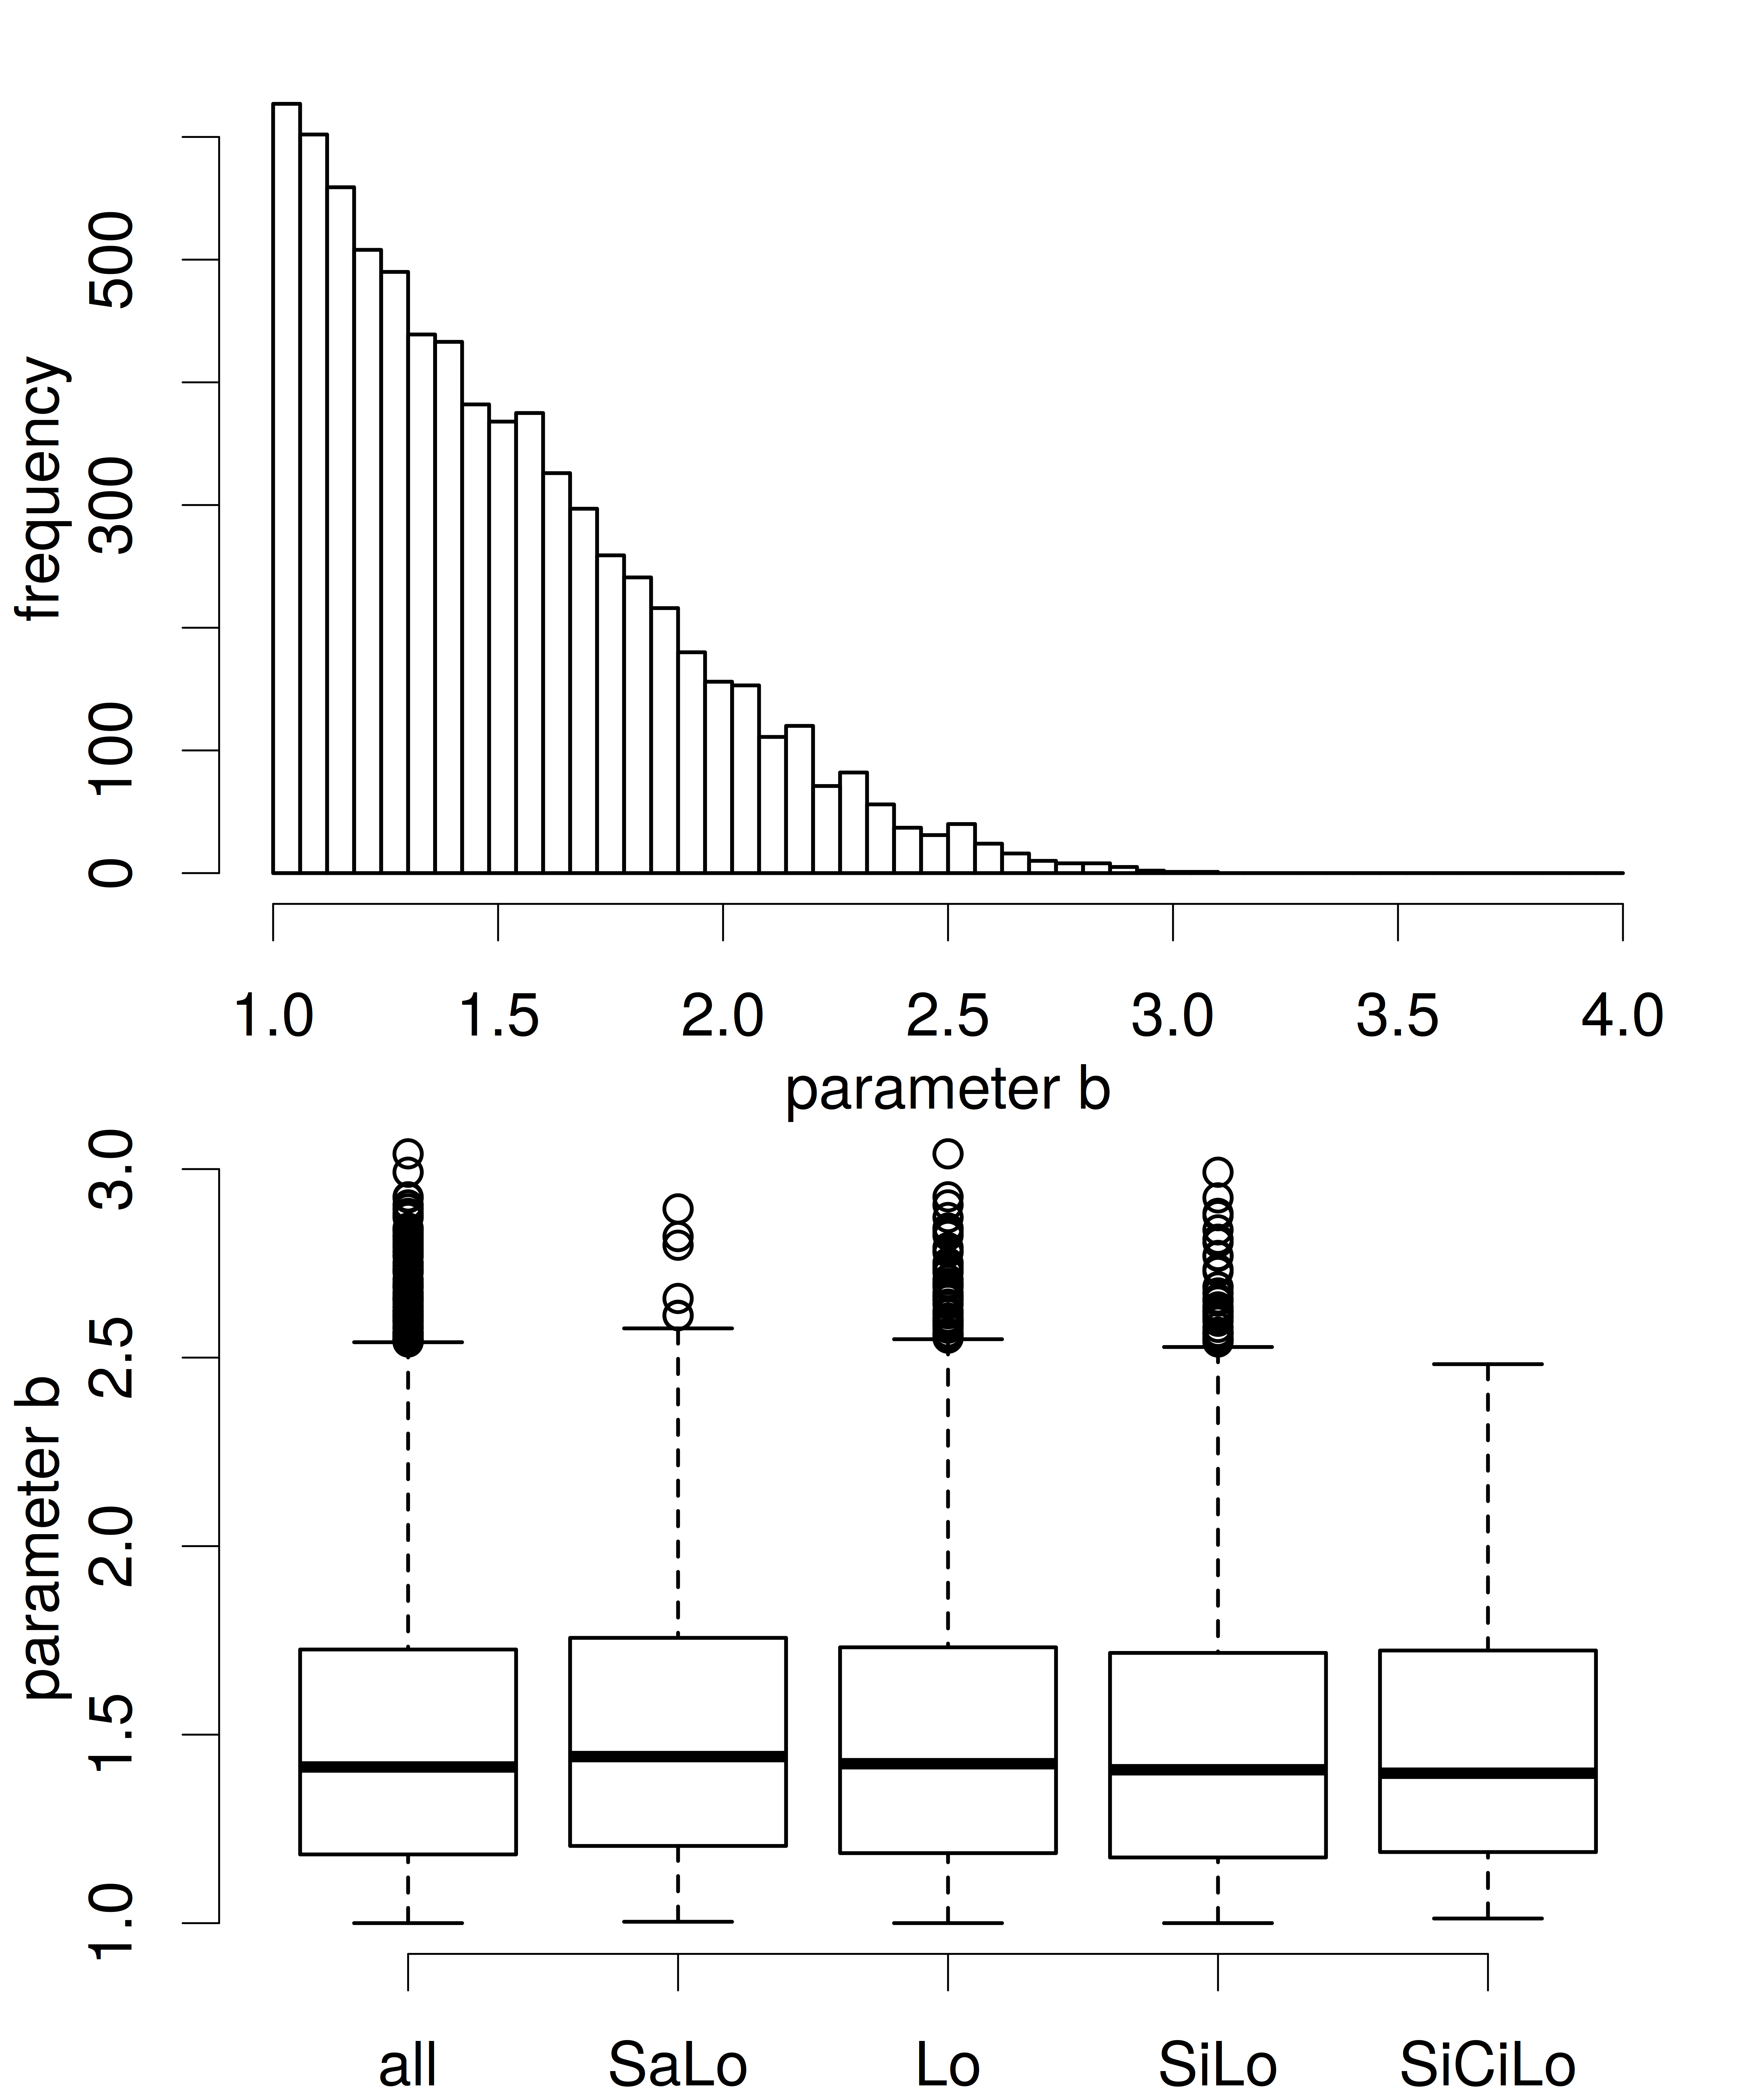
\includegraphics[width = \textwidth]{obr/mc_b.png}
            {\it ufh asdjfh aldksjfhlaskdjhf laksdjhf ladsjkfh }
        \end{column}
        \begin{column}{0.25\textwidth}
            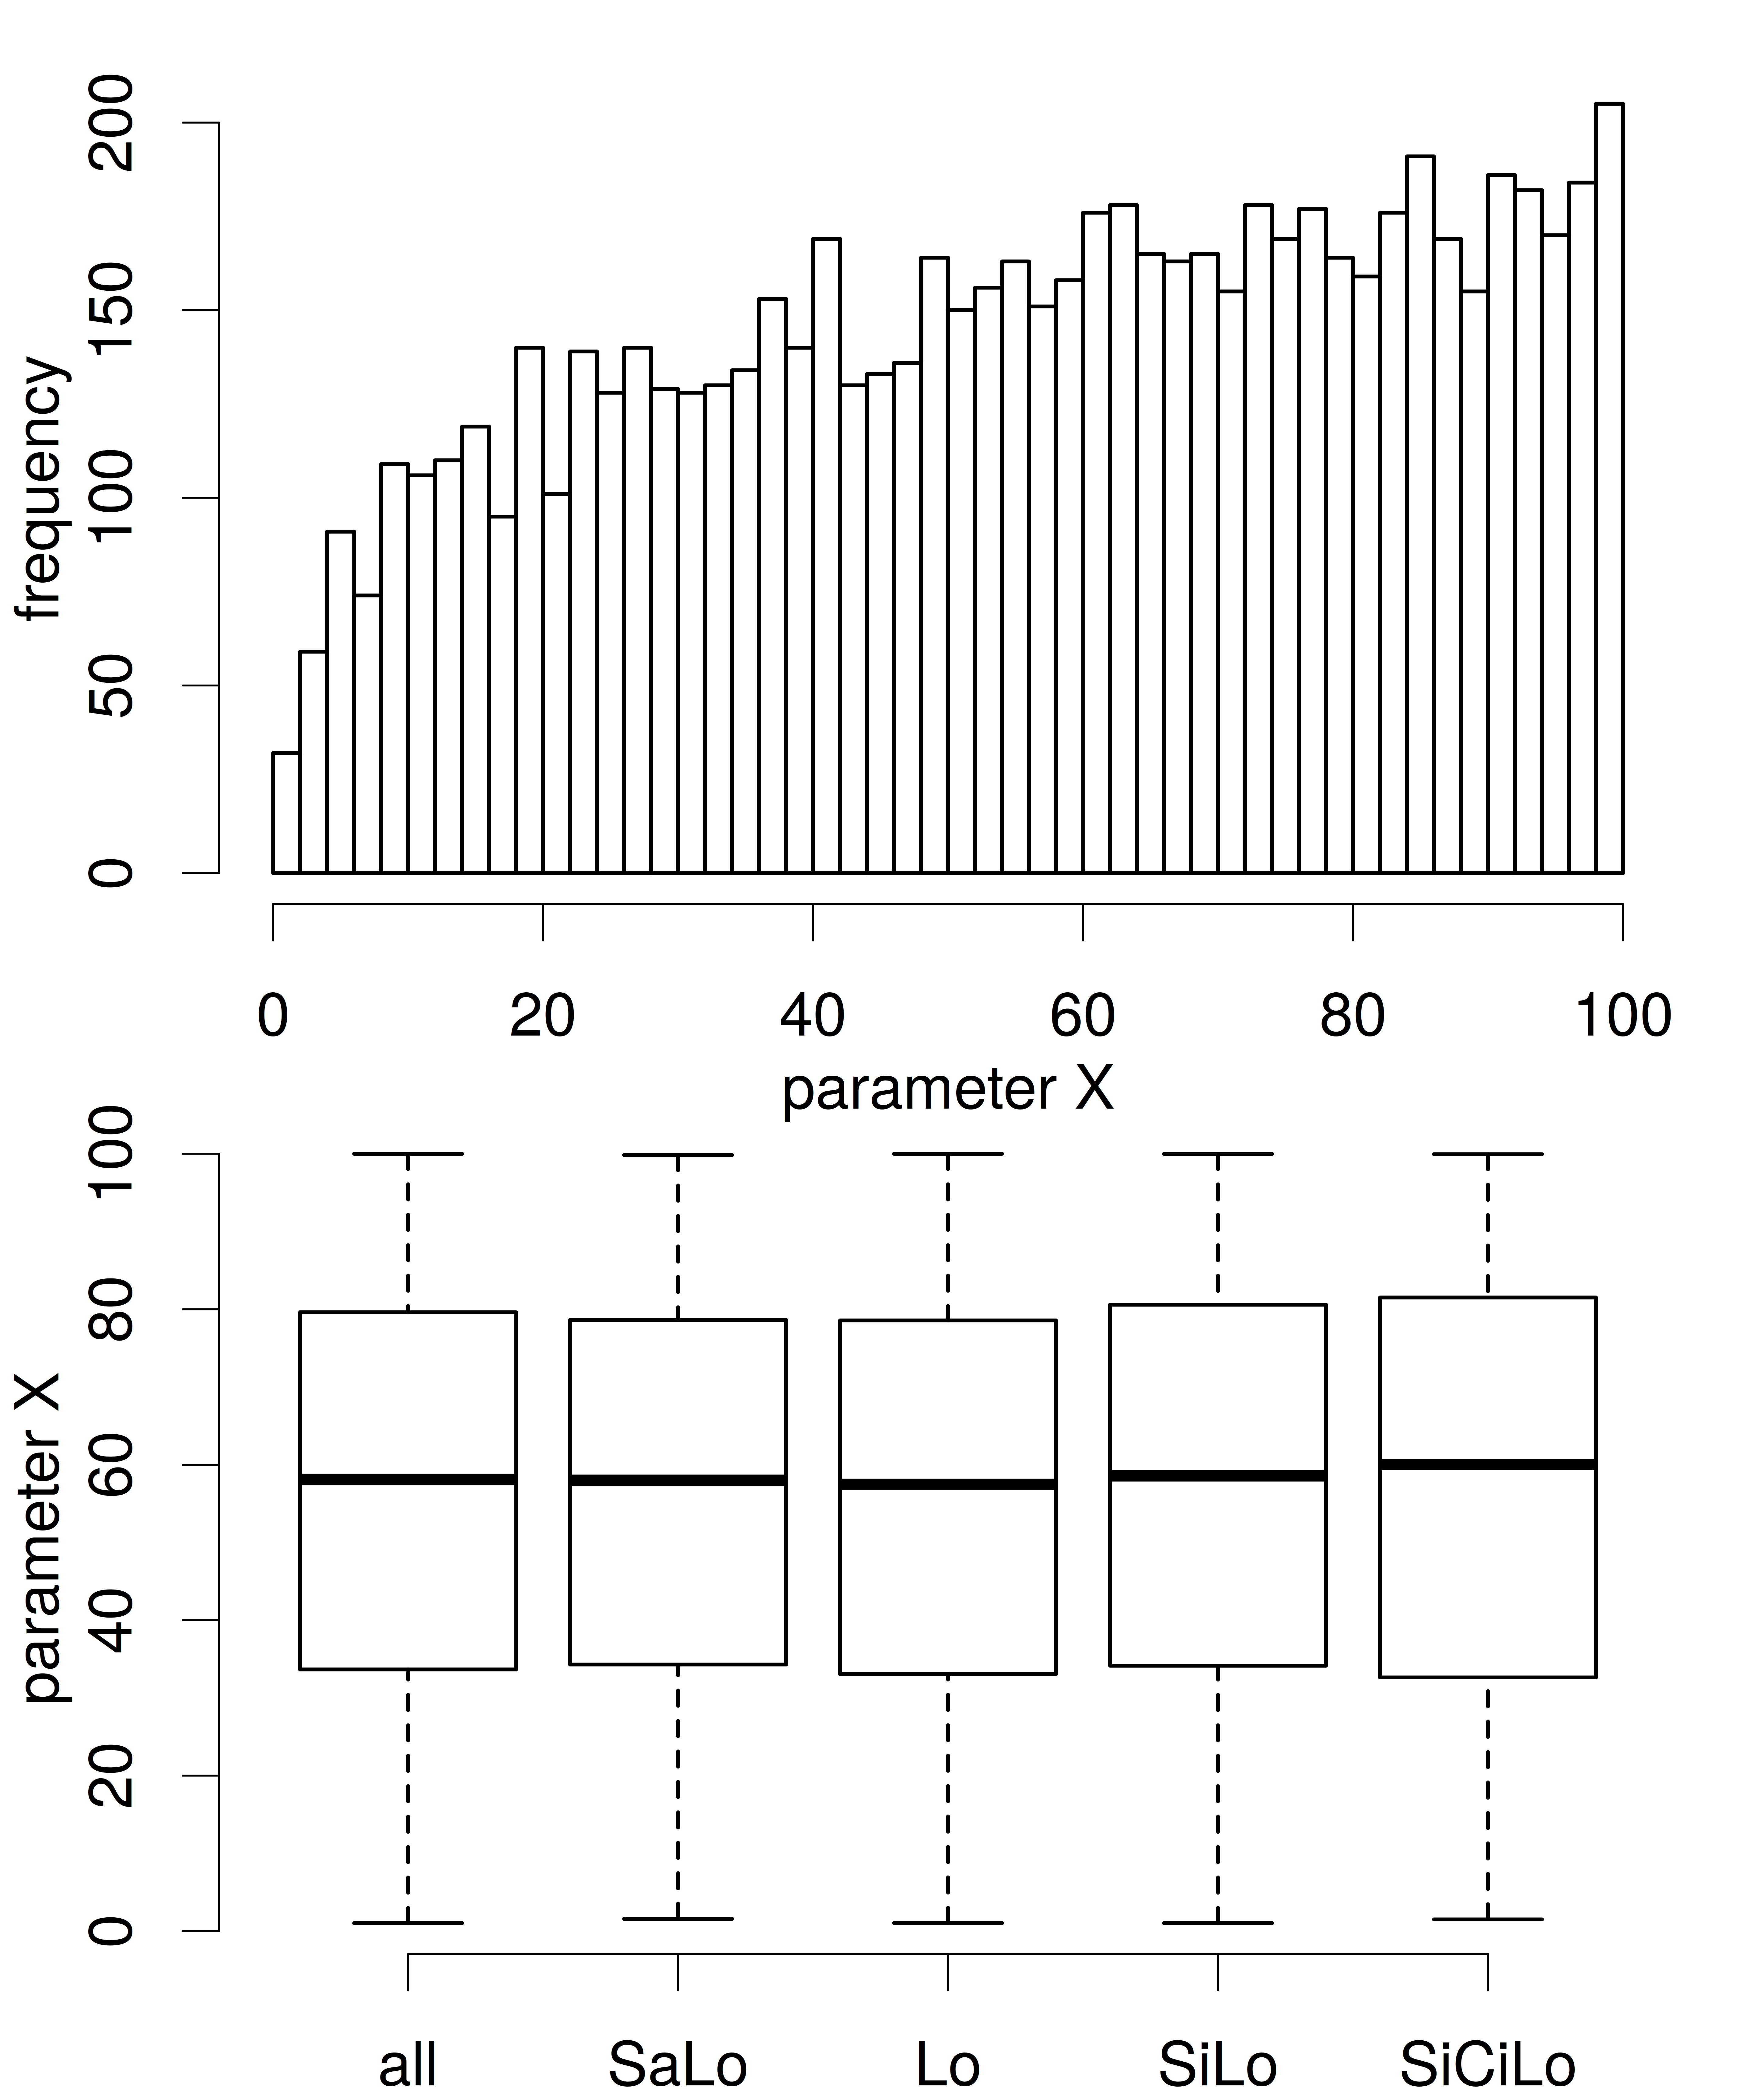
\includegraphics[width = \textwidth]{obr/mc_x.png}
            {\it ufh asdjfh aldksjfhlaskdjhf laksdjhf ladsjkfh }
        \end{column}
        \begin{column}{0.25\textwidth}
            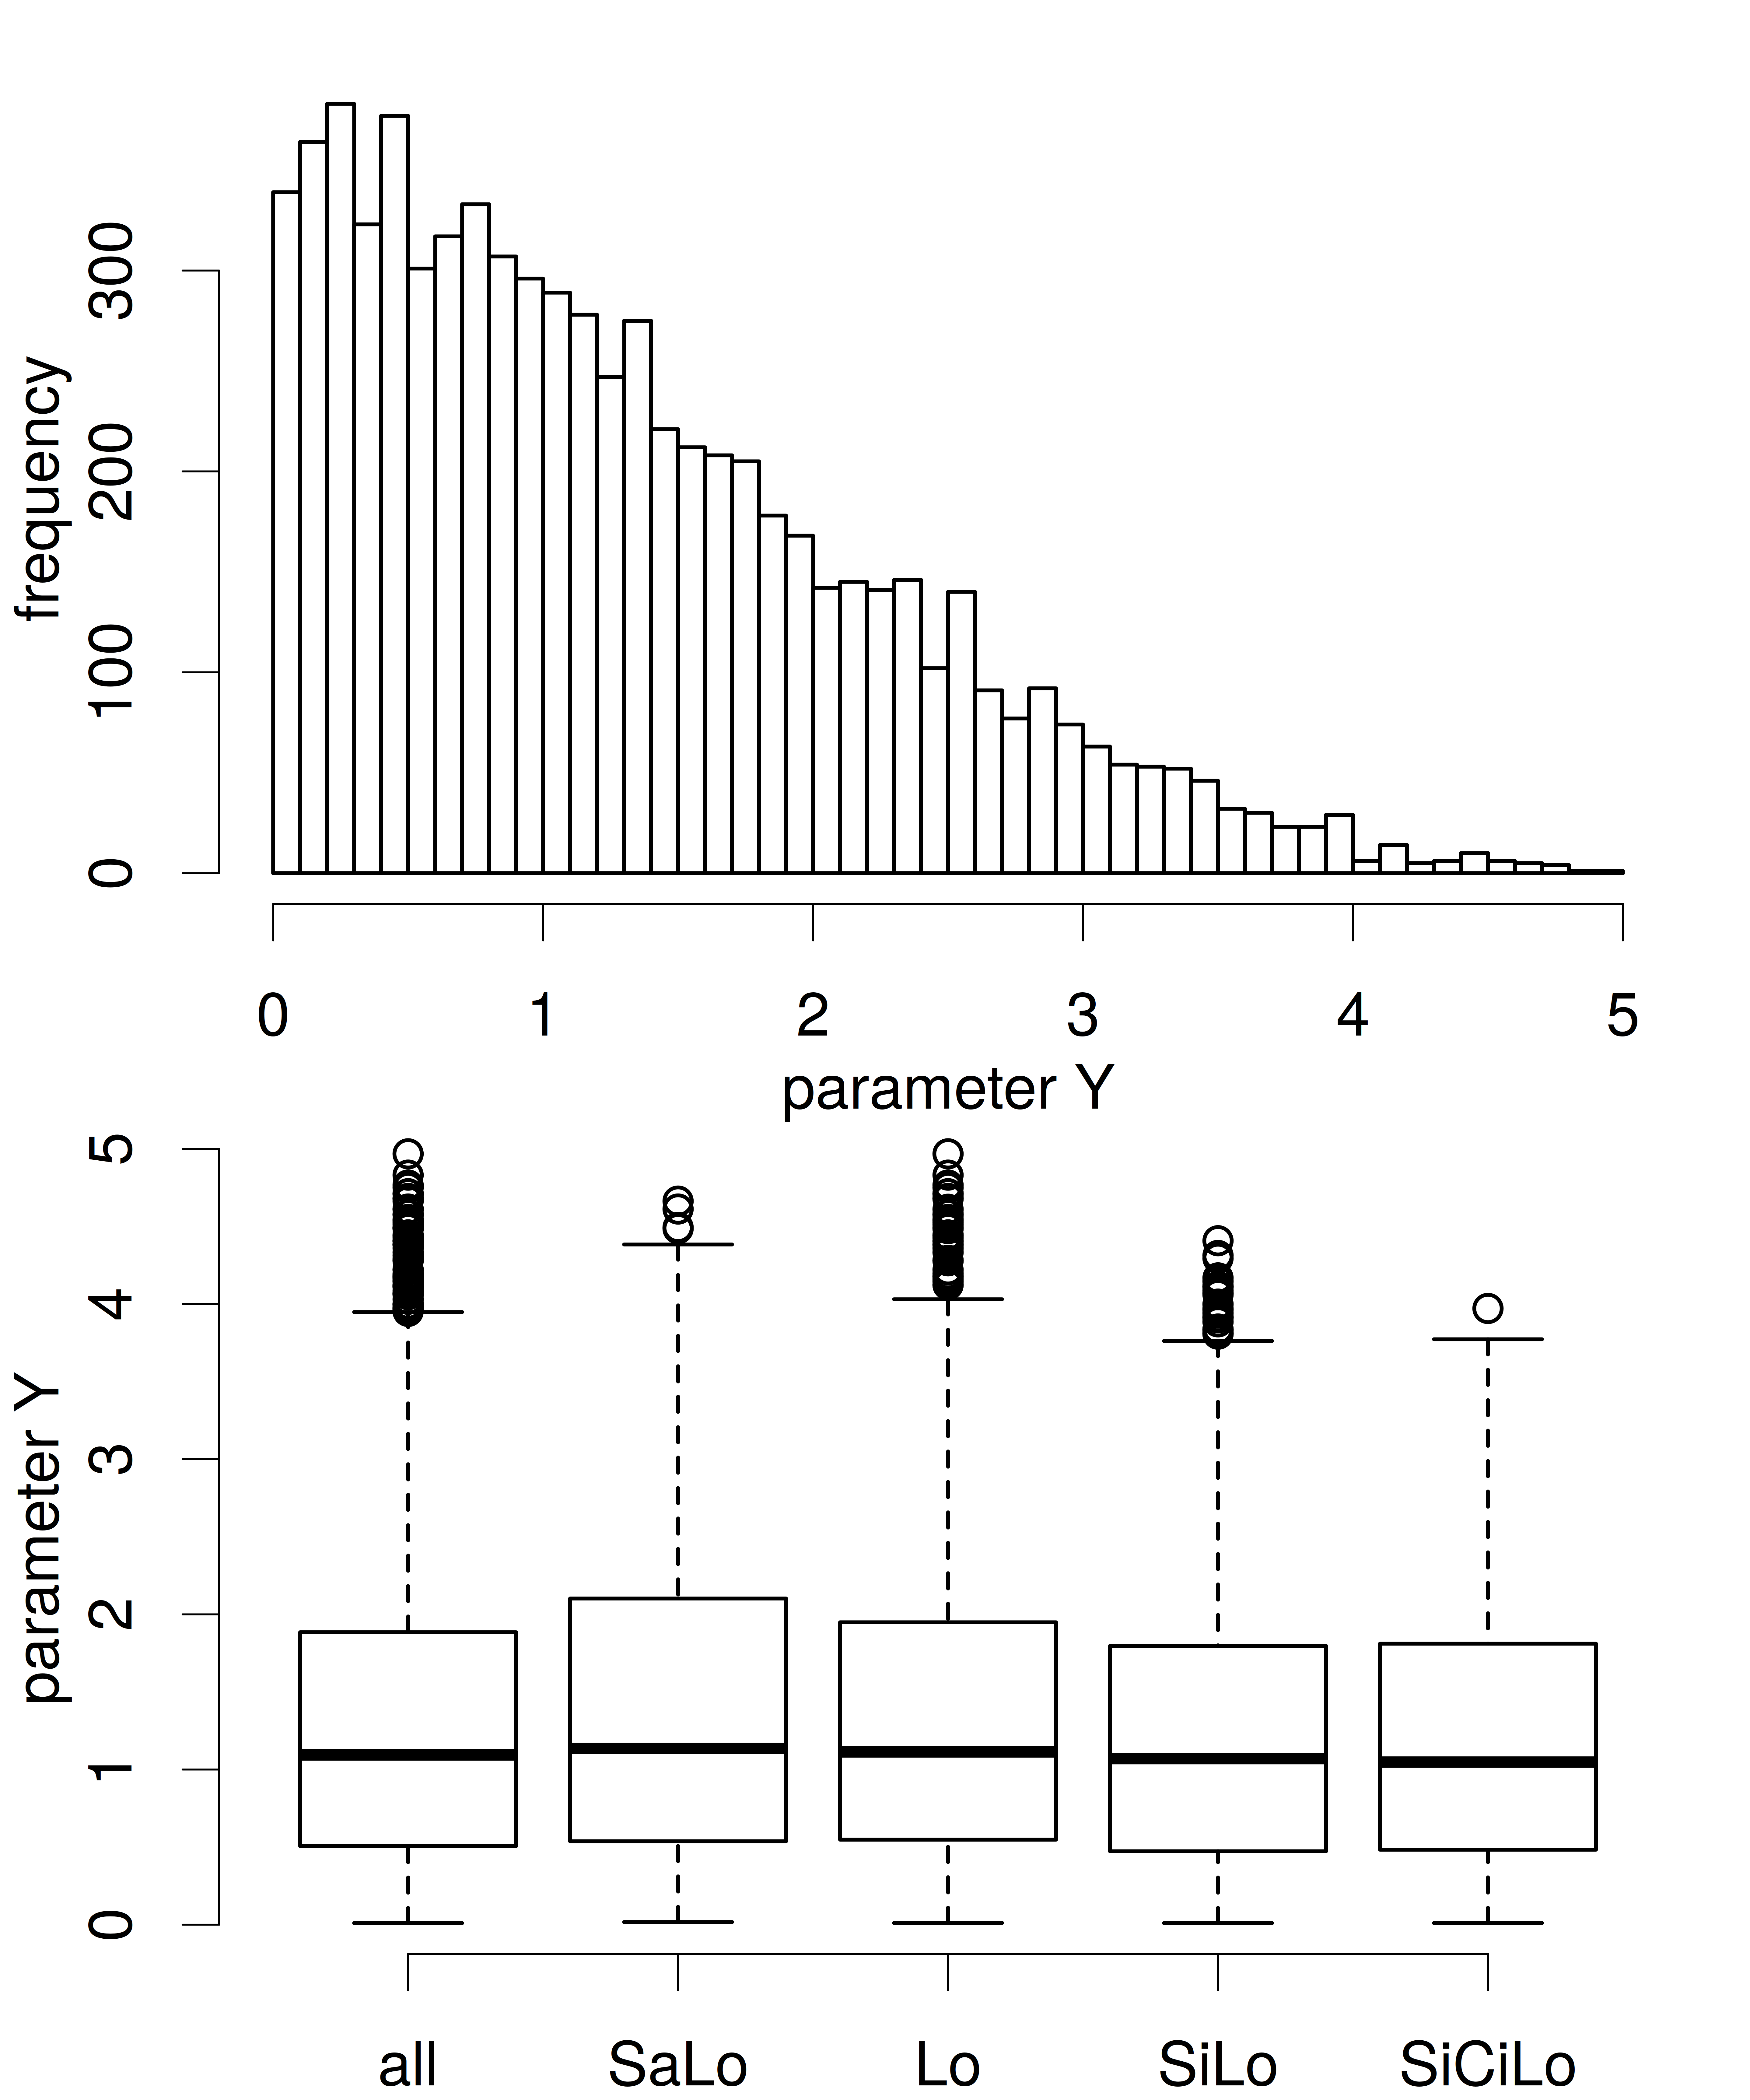
\includegraphics[width = \textwidth]{obr/mc_y.png}
            {\it ufh asdjfh aldksjfhlaskdjhf laksdjhf ladsjkfh }
        \end{column}
    \end{columns}
\end{block}















